% --------------------------------------------------------------
% This is all preamble stuff that you don't have to worry about.
% Head down to where it says "Start here"
% --------------------------------------------------------------
 
\documentclass[12pt]{article}

\usepackage{courier}
\usepackage{color}
\usepackage{listings}
\usepackage[square,numbers]{natbib}
\usepackage{tabls}
\usepackage{graphicx}
\usepackage{subcaption}
\usepackage{pdfpages}
\usepackage{mathtools}

\definecolor{dkgreen}{rgb}{0,0.6,0}
\definecolor{gray}{rgb}{0.5,0.5,0.5}




\lstset{language=python,
   basicstyle=\ttfamily,
   keywordstyle=\color{blue},
   commentstyle=\color{dkgreen},
   stringstyle=\color{red},
   numbers=left,
   numberstyle=\tiny\color{gray},
   stepnumber=1,
   numbersep=10pt,
   backgroundcolor=\color{white},
   tabsize=4,
   showspaces=false,
   showstringspaces=false}
 
\usepackage[margin=1in]{geometry} 
\usepackage{amsmath,amsthm,amssymb}
\usepackage{verbatim}
\usepackage{algpseudocode,algorithm}
\usepackage{setspace}

\newcommand{\ihat}{\ensuremath{\hat{\textbf{\i}}}}
\newcommand{\keff}{\ensuremath{k_{\mathrm{eff}}}}
\newcommand{\jhat}{\ensuremath{\hat{\textbf{\j}}}}
\newcommand{\lline}{\noindent\makebox[\linewidth]{\rule{\textwidth}{0.4pt}}}
\newcommand{\N}{\mathbb{N}}
\newcommand{\Z}{\mathbb{Z}}
\newcommand{\deriv}[2]{\frac{\mathrm{d} #1}{\mathrm{d} #2}}
\newcommand{\pderiv}[2]{\frac{\partial #1}{\partial #2}}
\newcommand{\bx}{\mathbf{X}}
\newcommand{\ba}{\mathbf{A}}
\renewcommand{\d}{\mathrm{d}}
\newcommand{\A}{\frac{(1-\alpha)}{2(1+\alpha)}}
\newcommand{\upl}{u_{\text{plane}}}
\newcommand{\upt}{u_{\text{point}}}
\newcommand{\D}{\Delta}
\newcommand{\ra}{\rightarrow}
\renewcommand{\SS}{\State}
 
\newenvironment{theorem}[2][Theorem]{\begin{trivlist}
\item[\hskip \labelsep {\bfseries #1}\hskip \labelsep {\bfseries #2.}]}{\end{trivlist}}
\newenvironment{lemma}[2][Lemma]{\begin{trivlist}
\item[\hskip \labelsep {\bfseries #1}\hskip \labelsep {\bfseries #2.}]}{\end{trivlist}}
\newenvironment{exercise}[2][Exercise]{\begin{trivlist}
\item[\hskip \labelsep {\bfseries #1}\hskip \labelsep {\bfseries #2.}]}{\end{trivlist}}
\newenvironment{problem}[2][Problem]{\begin{trivlist}
\item[\hskip \labelsep {\bfseries #1}\hskip \labelsep {\bfseries #2:}]\hspace{0.3in}\newline\newline}{\end{trivlist}}
\newenvironment{question}[2][Question]{\begin{trivlist}
\item[\hskip \labelsep {\bfseries #1}\hskip \labelsep {\bfseries #2.}]}{\end{trivlist}}
\newenvironment{corollary}[2][Corollary]{\begin{trivlist}
\item[\hskip \labelsep {\bfseries #1}\hskip \labelsep {\bfseries #2.} ]}{\end{trivlist}}
\newenvironment{problem*}[1][Problem]{\begin{trivlist}
\item[\hskip \labelsep {\bfseries #1} {\hspace{-0.2em}\bfseries:}]}{\end{trivlist}}
\newenvironment{solution}[1][Solution]{\begin{trivlist}
\item[\hskip \labelsep {\bfseries #1} {\hspace{-0.2em}\bfseries:}]\hspace{0.3in}\newline}{\end{trivlist}}
\newenvironment{solnum}[2][Solution]{\begin{trivlist}
\item[\hskip \labelsep {\bfseries #1}\hskip \labelsep {\bfseries #2:}]\hspace{0.3in}\newline\newline}{\end{trivlist}}
\newcommand{\iso}[2]{\ensuremath{^{#2}\text{#1}}}
\newcommand{\nubar}{\ensuremath{\overline{\nu}}}
 
\begin{document}
 
% --------------------------------------------------------------
%                         Start here
% --------------------------------------------------------------
 
\title{Homework 4}%replace X with the appropriate number
\author{Simon Bolding\\ %replace with your name
NUEN 629} %if necessary, replace with your course title
 
\maketitle

\clearpage

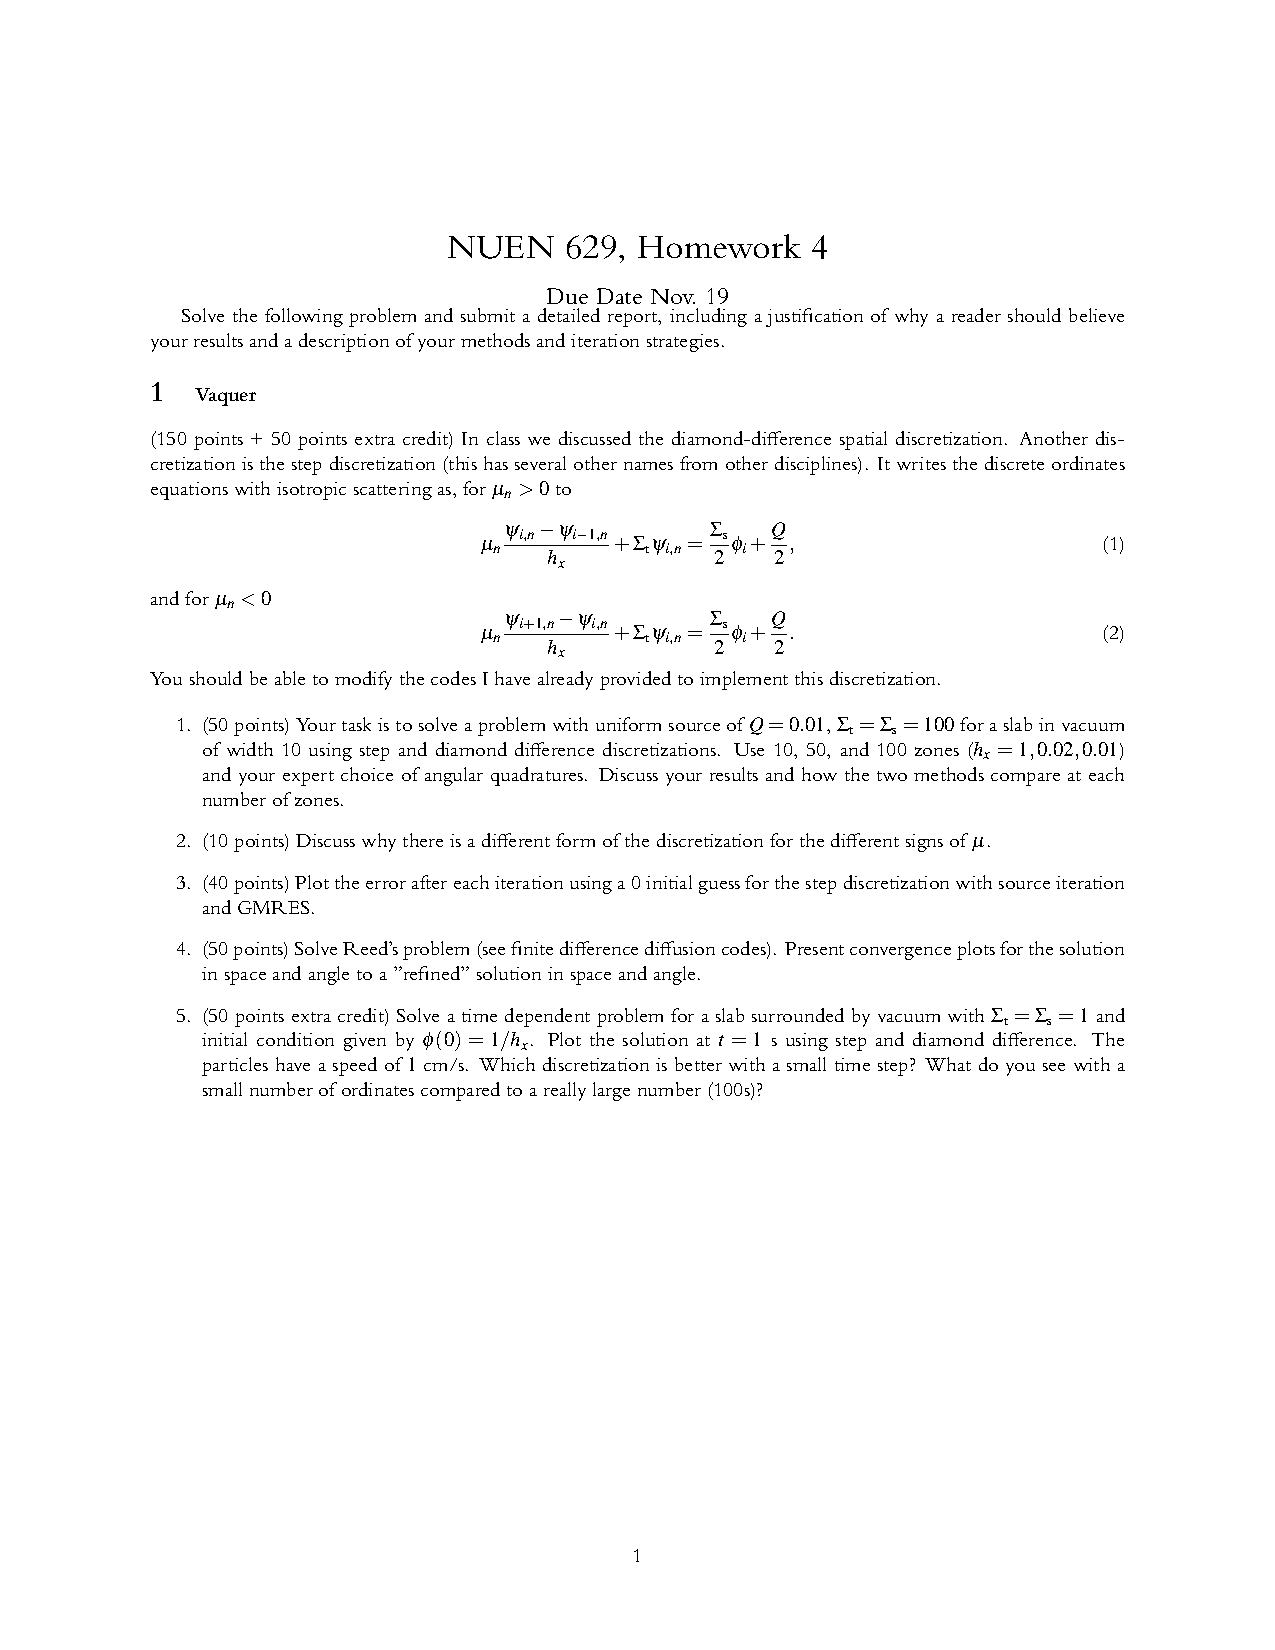
\includepdf{Homework4.pdf}

\begin{solnum}{1-1}

To modify the provided code to use the step discretization, essentially only the
1DSweep function needs to be modified.  For example, for a positive direction of
$\mu_n$ the flux in the $i$-th cell is, for the $k-th$ sweep,
\begin{equation}
    \psi^{(k+1)}_{i,n} = \frac{\frac{1}{2}\left(\phi^{(k)}_i + Q\right) +
    \frac{\mu_n}{h_x}\psi^{(k+1)}_{i-1,n}}{\Sigma_t + \frac{\mu_n}{h_x}},
\end{equation}
where $\psi_{i-1,n}$ is either defined by the boundary conditon, i.e., $\psi_{0} =
f(\mu_n)$, or is known from solution of the previous cell in the sweep. The negative
direction sweep is defined analogously. A correction was also made to the diamond
difference sweep code.

For the given problem parameters, source iteration was too slow to converge because
the scattering ratio is $c=1$, so the
GMRES solver was used for both spatial discretizations.  For one case GMRES was
verified to converge to the same solution as source iteration.  A plot of the
different solutions for the different resolutions and spatial discretizations is
given below, for $N=16$ angles, in Fig.~\ref{fig1}. On
the finest mesh, increasing to $N=24$ had no visible effect on the solution.  The
step discretization does not get the asymptotic diffusion limit, so the solution
produces inaccurate and variable results for the different refinement levels.  The
DD solution appears to be converging correctly.  

 Also plotted below is an analytic diffusion 
solution to the same problem using Mark Boundary conditions, compared
to the DD solution and step with a very fine mesh. For this problem diffusion theory should be accurate, particularly
several diffusion lengths from the boundary.  Although the mesh size  for the step
discretization is fine to the $O(1/\Sigma_t)$, the
solution still disagrees, although it does appear to be converging towards the
correct solution.  This seems to be due to the fact that it is a pure
scattering solution.  Keeping the same thickness but with a small amount of
absorption showed better agreement.

\begin{figure}[h!]
    \centering
    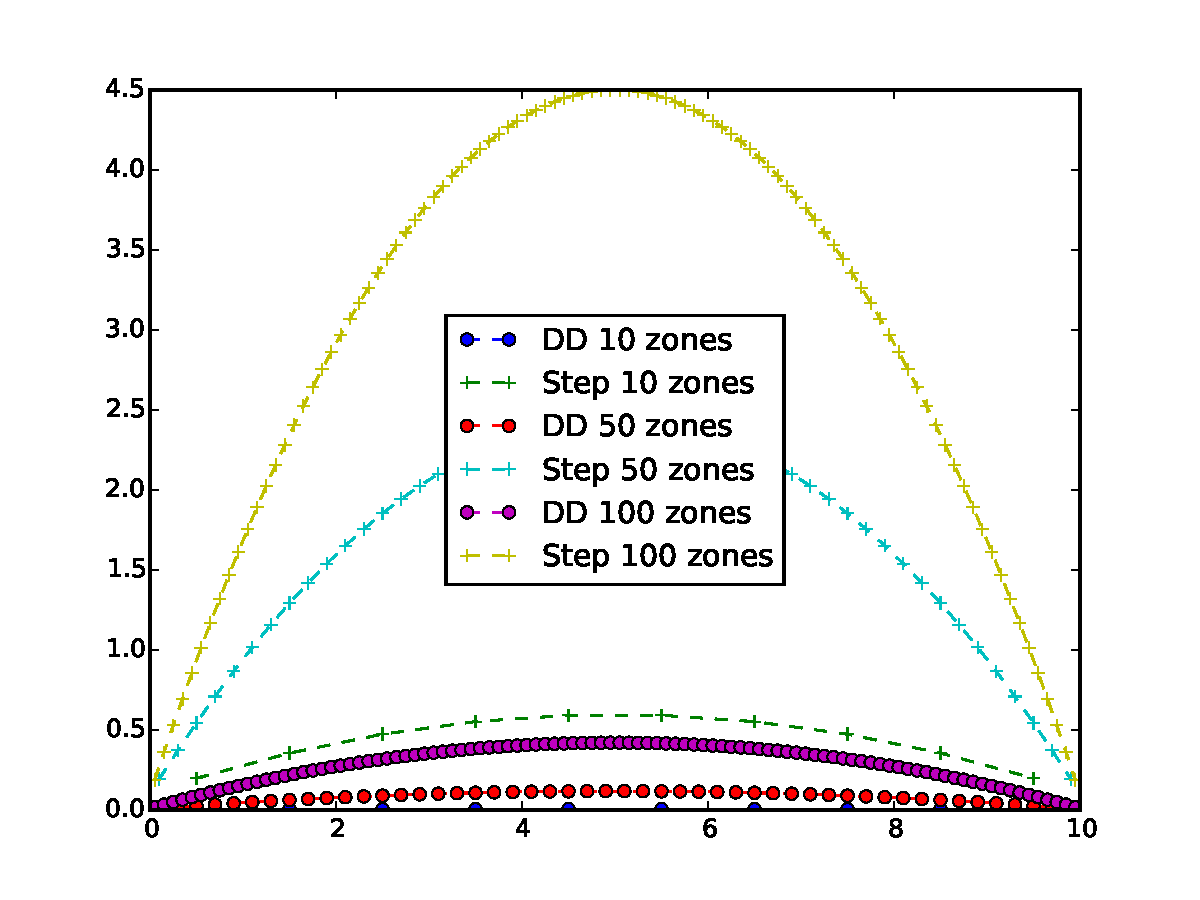
\includegraphics[width=0.5\textwidth]{prob1.pdf}
    \caption{Comparison of step and DD spatial discretizations for different numbers
        of zones.\label{fig1}}
\end{figure}
\begin{figure}[h!]
    \centering
    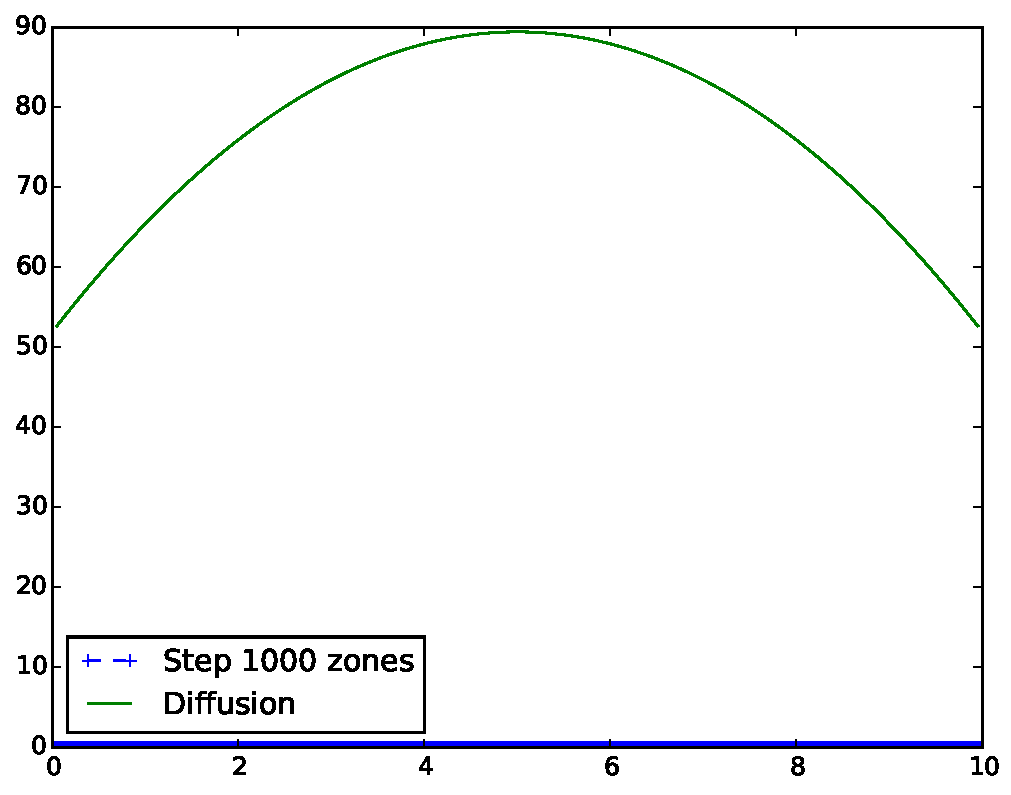
\includegraphics[width=0.5\textwidth]{diff.pdf}
    \caption{Comparison of analytic diffusion theory, diamond difference, and a
    highly refined step solution.}
\end{figure}
    

\end{solnum}

\clearpage

\begin{solnum}{1-2}

The different forms of the discretization are result of the solution being generally
undefined at the faces of cells, due to the discontinuity of the solution at cell
edges.  A closure of some kind must be defined because even in the weak-form we need
a value for $\psi$ on the face.  The given equations define $\psi$ on the face using the upwind closure, which attempts to numerically
propagate information in the physical direction of flow, based on the characteristic
flow of information in each direction.  This, in theory, resolves strong spatial
gradients with higher physical accuracy.  This closure also provides stability to the
equations, which could demonstrate oscillations with a poor choice of closure.

\end{solnum}

\begin{solnum}{1-3}

For convenience, slightly different measures of convergence error are compared
between source iteration and GMRES. The GMRES solver returns the relative residual
which demonstrates how well the solution is satisfied,
whereas for source iteration the relative change between iterations of
the scalar flux $(\phi^k - \phi^{k-1})/\phi^k$ is used.  GMRES with no restart and a
restart of 20 are compared. Results are shown for the case of 100 cells and 16
angles.  As seen in the figure below, GMRES without restart quickly converges after
an initial slow start.  Because the problem is slowly converging, most of the krylov
space needs to be formed before the error is rapidly converged upon.  Restarting
limits the space that is projected onto, leading to a steady, slower convergence.
Source iteration is very slow to converge.  Initially source iteration looks better
than GMRES.  This is probably partially due to the difference in errors.  In slowly
converging systems, the difference in solution is not an accurate estimate of the
error, and should really take into account the dominance ratio $\rho$ as
$1/(1-\rho)(\phi^k - \phi^{k-1})$.
\begin{figure}[h!]
    \centering
    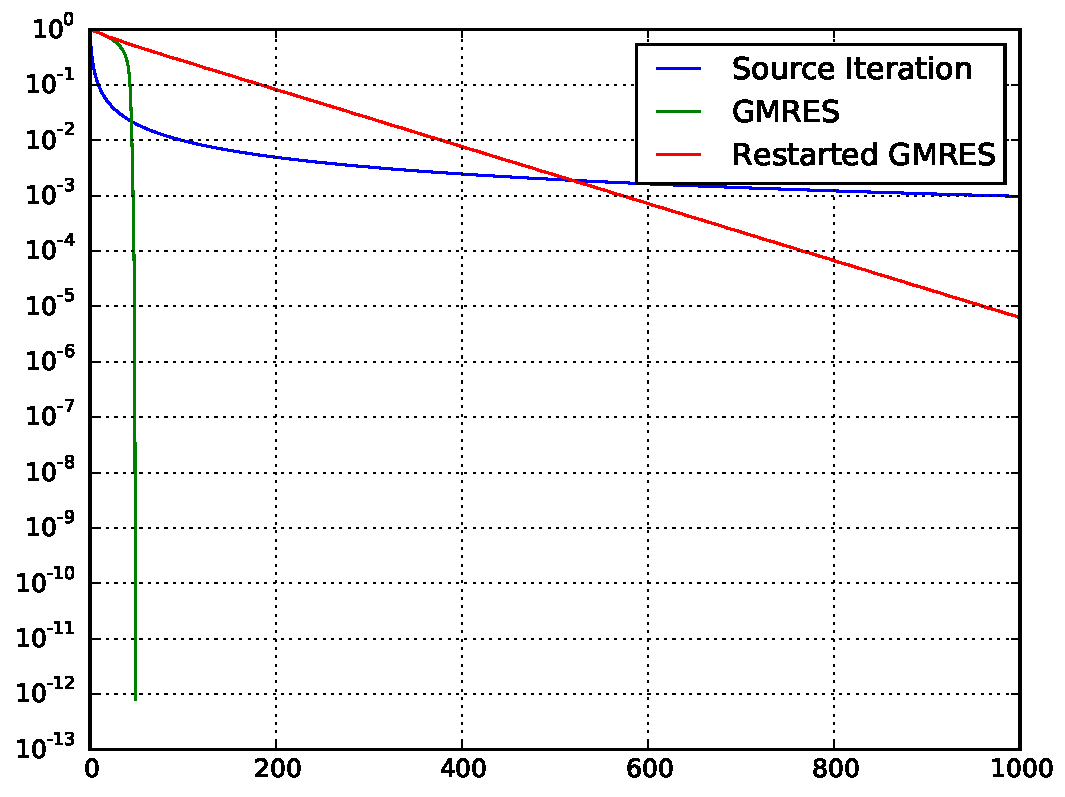
\includegraphics[width=0.5\textwidth]{err.pdf}
    \caption{Convergence rates of scattering iterations for source iteration and
        GMRES for Problem 1-1.}
\end{figure}

\end{solnum}

\clearpage

\begin{solnum}{1-4}

Plots of the solution to Reed's problem for DD and step discretization are given in
Fig.~\ref{reed1}. Step has trouble resolving the high spatial variation, particularly
in the scattering and source dominated region, and spreads
out the answer.  However, in the optically thick, pure absorber regions, DD
demonstrates spurious oscillations. This is because diamond difference is not
``$L$-stable'', similar to crank nicolson.  For
the case of a pure absorber you can write the amplitude between cells as
\begin{equation*}
    \psi_{i+1/2} = \left(\frac{1 - \frac{\Sigma \Delta x}{2\mu}}{1 + \frac{\Sigma
    \Delta x}{2\mu}} \right)\psi_{i-1/2}
\end{equation*}
which is always stable because the quantity in parenthesis has magnitude less than
one, but the quantity does not to go 0 as $\Sigma \Delta x$ goes to infinity.
If $\frac{\Sigma \Delta x}{2\mu} > 1$, then the amplification will be negative, which
would result in oscillations from cell to cell.

For error convergence an approximate $L2$ error was computed as
\begin{equation}
    e^{(k)} = \sqrt{\sum_{i=0}^{N_{cells}} (\phi_{i}^{(k)} -
    \phi^{\text{ref}}(x_i))^2 \Delta x_i         }
\end{equation}
where $\phi_i$ is the cell average and $\phi^{\text{ref}}(x_i)$ is evaluated at the
cell center of $i$ using a cubic interpolation based on the finest mesh solution.
The fine solution is taken to be 600 $x$ cells and $120$ directions.  Plots of the
error convergence can be seen below.  The
convergence in space is not very consistent, although it does appear to be converging
towards the refined solution.  This is partially due to the discontinuities in
material properties and that the number of cells with different properties varies as
the mesh sizes change.  The convergence in angle shows a consistent and convergent
behavior for both spatial discretizations.
\begin{figure}[h!]
    \centering
    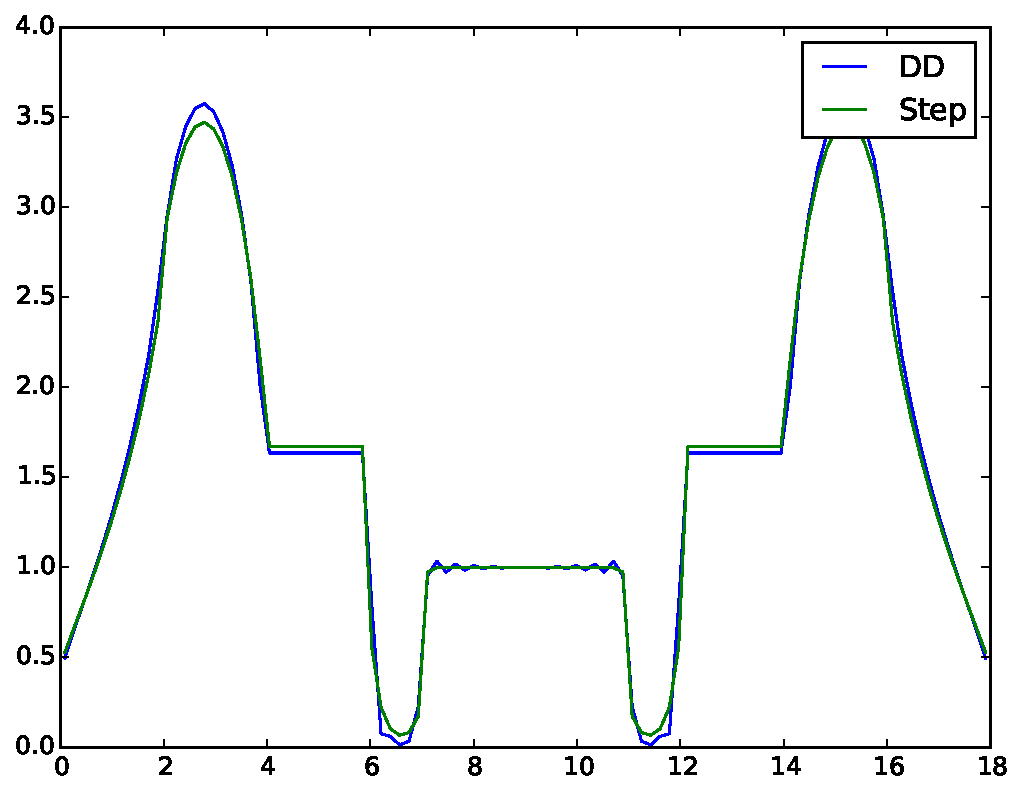
\includegraphics[width=0.5\textwidth]{reed.pdf}
    \caption{Solutions for Reed's problem.}
\end{figure} 
\begin{figure}[h!]
    \centering
    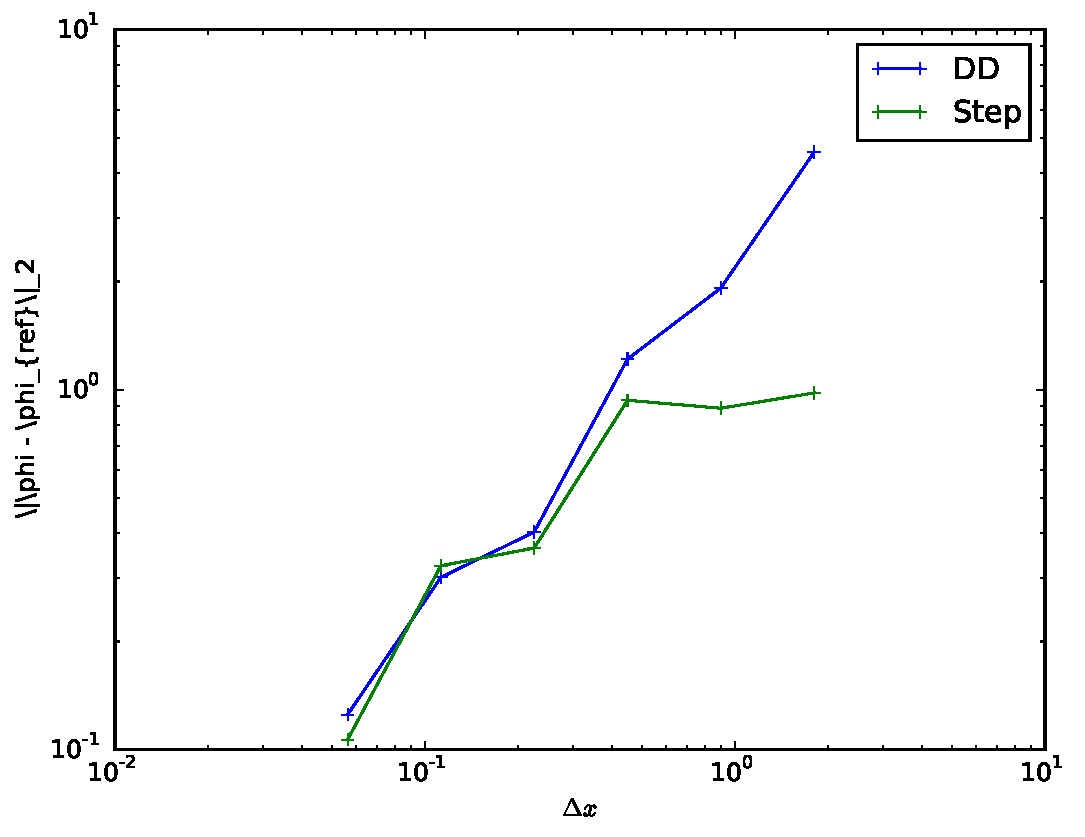
\includegraphics[width=0.5\textwidth]{err_reedx.pdf}
    \caption{Convergence in space for Reed's problem.}
\end{figure} 
\begin{figure}[h!]
    \centering
    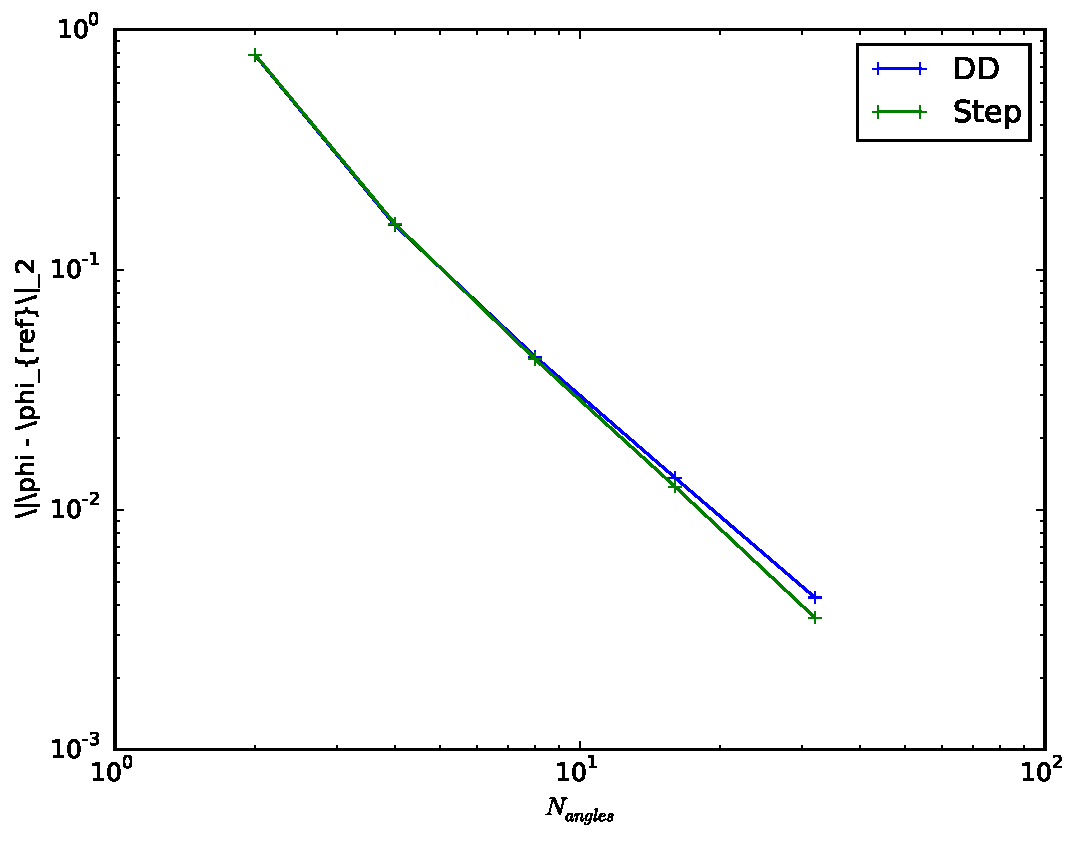
\includegraphics[width=0.5\textwidth]{err_reedmu.pdf}
    \caption{Convergence in angle for Reed's problem.}
\end{figure} 

\end{solnum}

\begin{solnum}{1-5}

The code was modified to account for a backward Euler time discretization.
The changes to the equations yield the simple changes 
\begin{align}
    \Sigma_t \rightarrow& \Sigma_t + \frac{1}{v\Delta t} \\
    q_n \rightarrow& q_n + \phi_i^{m+1}{2} + \frac{1}{v\Delta t}\psi_{n,i}^{m}
\end{align}
for the $m$-th time step. The angular flux is stored between solves.  The old angular flux is used as the guess
for the scattering source iteration, which significantly improves convergence in
later time steps.  The angular flux in the cell at the center of the slab is
initialized to $1/(2h_x)$ for all $\mu_n$.

A plot of the solution for both discretizations with 200 spatial
cells is shown below for two different time steps. The DD solution is inaccurate in
both cases, and for the short time-step DD demonstrates severe oscillations. These
oscillations result once the effective $\Sigma_t$ becomes too large due to the
$1/(v\Delta t)$ term.  Even though step is generally a more diffusive discretization, it is the more
accurate choice in this case as DD oscillates and goes negative, although it appears
DD is getting a more accurate location of the wave.  Both discretizations agree on the location of the
wave-front, although the step solution for $\Delta t\leq 0.01$ has a slightly faster
wave at the edge due to the diffusive nature of the discretization. As the time step
goes from $0.01$ s to $0.002$ s, the wave-front does not get sharper for step, where
as it does for DD (the DD seems more accurate in this case).  This is because the spatial discretization error is dominating,
and more mesh cells are needed.  It is noted that unless $\Sigma_t$ is very large or $\Delta t$ is very
small, the Backward Euler has significant artificial diffusion in the time variable,
which is part of the cause of the difference in shape of the solutions on the very coarse
time-step.
For this problem 200 directions were needed to eliminate
any spikes in the solution that occured from angular discretization error rather than
spatial resolution issues.

Plotted below is the solution for various numbers of angles for the step
discretization. For smaller number of angles there is noticable ray effects as the
particles advect only in specific directions at the same speed, producing an artificially fast
wavefront with spikes present, particularly noticeable for the case of 2 angles. As more angles are added, the wave
front approach a more physically accurate solution. 
\begin{figure}[h!]
    \centering
    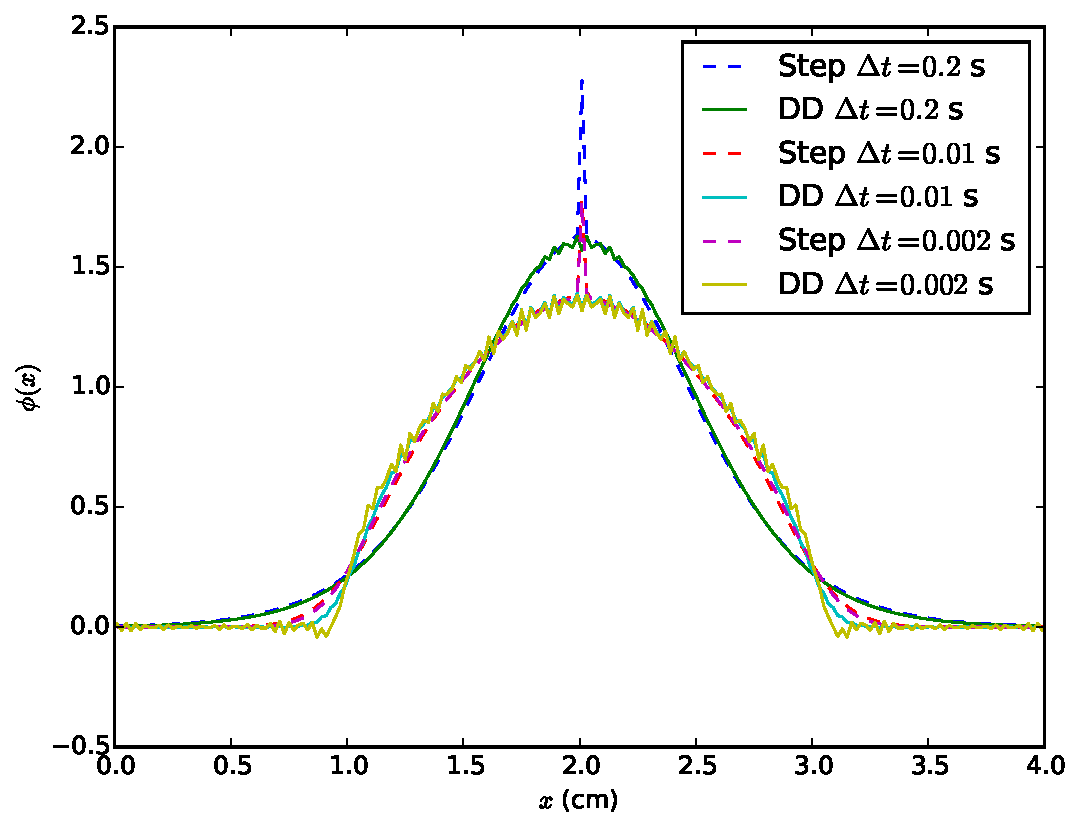
\includegraphics[width=0.5\textwidth]{time_dep_steps.pdf}
    \caption{Comparison of spatial discretizations after 1 s, for different time step
    sizes.}
\end{figure} 
\begin{figure}[h!]
    \centering
    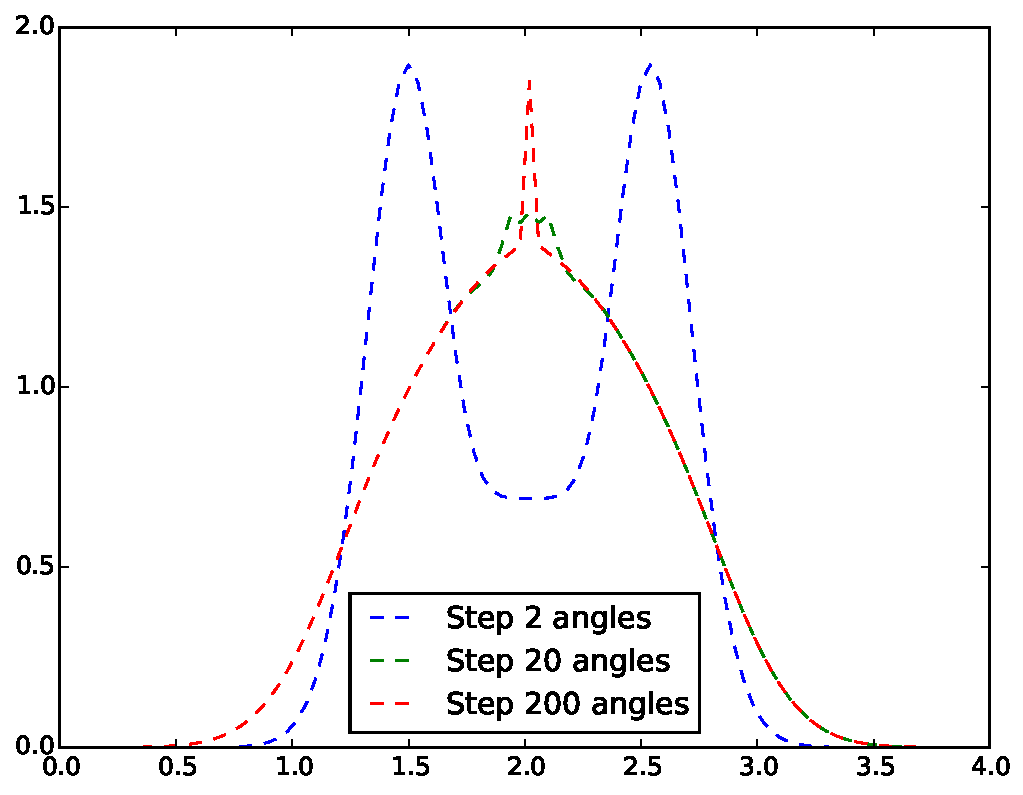
\includegraphics[width=0.5\textwidth]{time_dep_angles.pdf}
    \caption{Comparison of step solutions for various numbers of quadrature
    directions.}
\end{figure} 


\end{solnum}

\clearpage
\subsubsection*{Code}
\lstinputlisting[basicstyle=\scriptsize]{SnSlab.py}

\end{document}

